\documentclass[../main.tex]{subfiles}

\begin{document}

\section{Results}


\subsection{Fluorescent Proteins}

With kind support from other sources (see section~\ref{sec:plaspri:plas}) we built up a library of many fluorescent protein-chemotaxis protein fusions. However, it was still necessary to exchange many of these. Many fluorescent proteins\myfootnote{CFP, YFP, BFP and further derivatives} are all derivatives of GFP through only a few amino acid substitutions\cite{tsien98}. In most modernly used GFP derivatives, these all lie between amino acid 64 and amino acid 206, inclusive. Therefore, through careful design of PCR primers Gibson assembly can be used to exchange one GFP derivative for another with the same set of primers (see section~\ref{sec:plaspri:pri}).

Primarily EYFP was used for the proteins being imaged. However, a monomeric form was required for anisotropy\cite{vaknin07}, requiring the mutation A206K. Another EYFP varaent, known as Venus, was described as being a better FRET receiver\cite{nagai02} as well as a generally improved fluorophore, and therefore ideal for our anisotropy experiments. However, only the monomeric EYFP variant was available to us, and we have not yet had time to perform the five amino acid substitutions required for Venus.

\subsection{Inducer Calibration}

Most fusion proteins were available, or could easily be made available, in both the pBAD33 or pTRC99a plasmid, induced by arabinose or IPTG respectively. As in some experiments we planned to induce two proteins using both, it was important to be able to balance the production of each, by performing inducer titres and timecourses. Three experiments were performed.

\paragraph{Inducement time.} Generally it is recommended to induce some time after inoculating fresh media with overnight cultures; however this is not necessary if the proteins being induced are not toxic. Two parallel growths were done, OD measurements taken every two hours, and images recorded 4 hours after induction and four hours after inoculation.
\begin{center}
\begin{tabular}{ccc}
t=0	&	Inoculate	&	Inoculate \& Induce\\
2	&	Induce	&\\
4	&	Image	&	Image\\
6	&	Image	&
\end{tabular}
\end{center}

\paragraph{Inducer Titre} A logarithmic course of inducer concentrations was checked for expression of the same fusion protein under different promoters.

\begin{center}
\begin{tabular}{cc}
\textbf{Arabinose}	&	\textbf{IPTG} 	\\
0.001\%	&	\SI{1}{\micro\Molar}\\
0.003\%	&	\SI{3}{\micro\Molar}\\
0.01\%	&	\SI{10}{\micro\Molar}\\
0.03\%	&	\SI{30}{\micro\Molar}\\
0.1\%	&	\SI{100}{\micro\Molar}\\

\end{tabular}
\end{center}

\paragraph{Time Course}	A selection of inducer concentration from the inducer titre were re-run with samples being removed and imaged at \SI{2}{\hour}, \SI{3}{\hour} and \SI{4}{\hour} to find optimal expression.
 

\subsection{Cluster Sizing using Image Processing}

The following section contains results from image processing based techniques as described in section~\ref{sec:methods:imageprocessing}.

\subsubsection{Epifluorescence Microscopy}
\label{sec:results:cs:epi}

These experiments were performed on a Nikon microscope on loan from the manufacturer. One image was taken each from a slide of cells prepared with and without cobalt.

\begin{figure}[h!]
\begin{center}
\subfloat[No cobalt, \(n=18, \mu=0.144, \sigma=0.070\)]{
	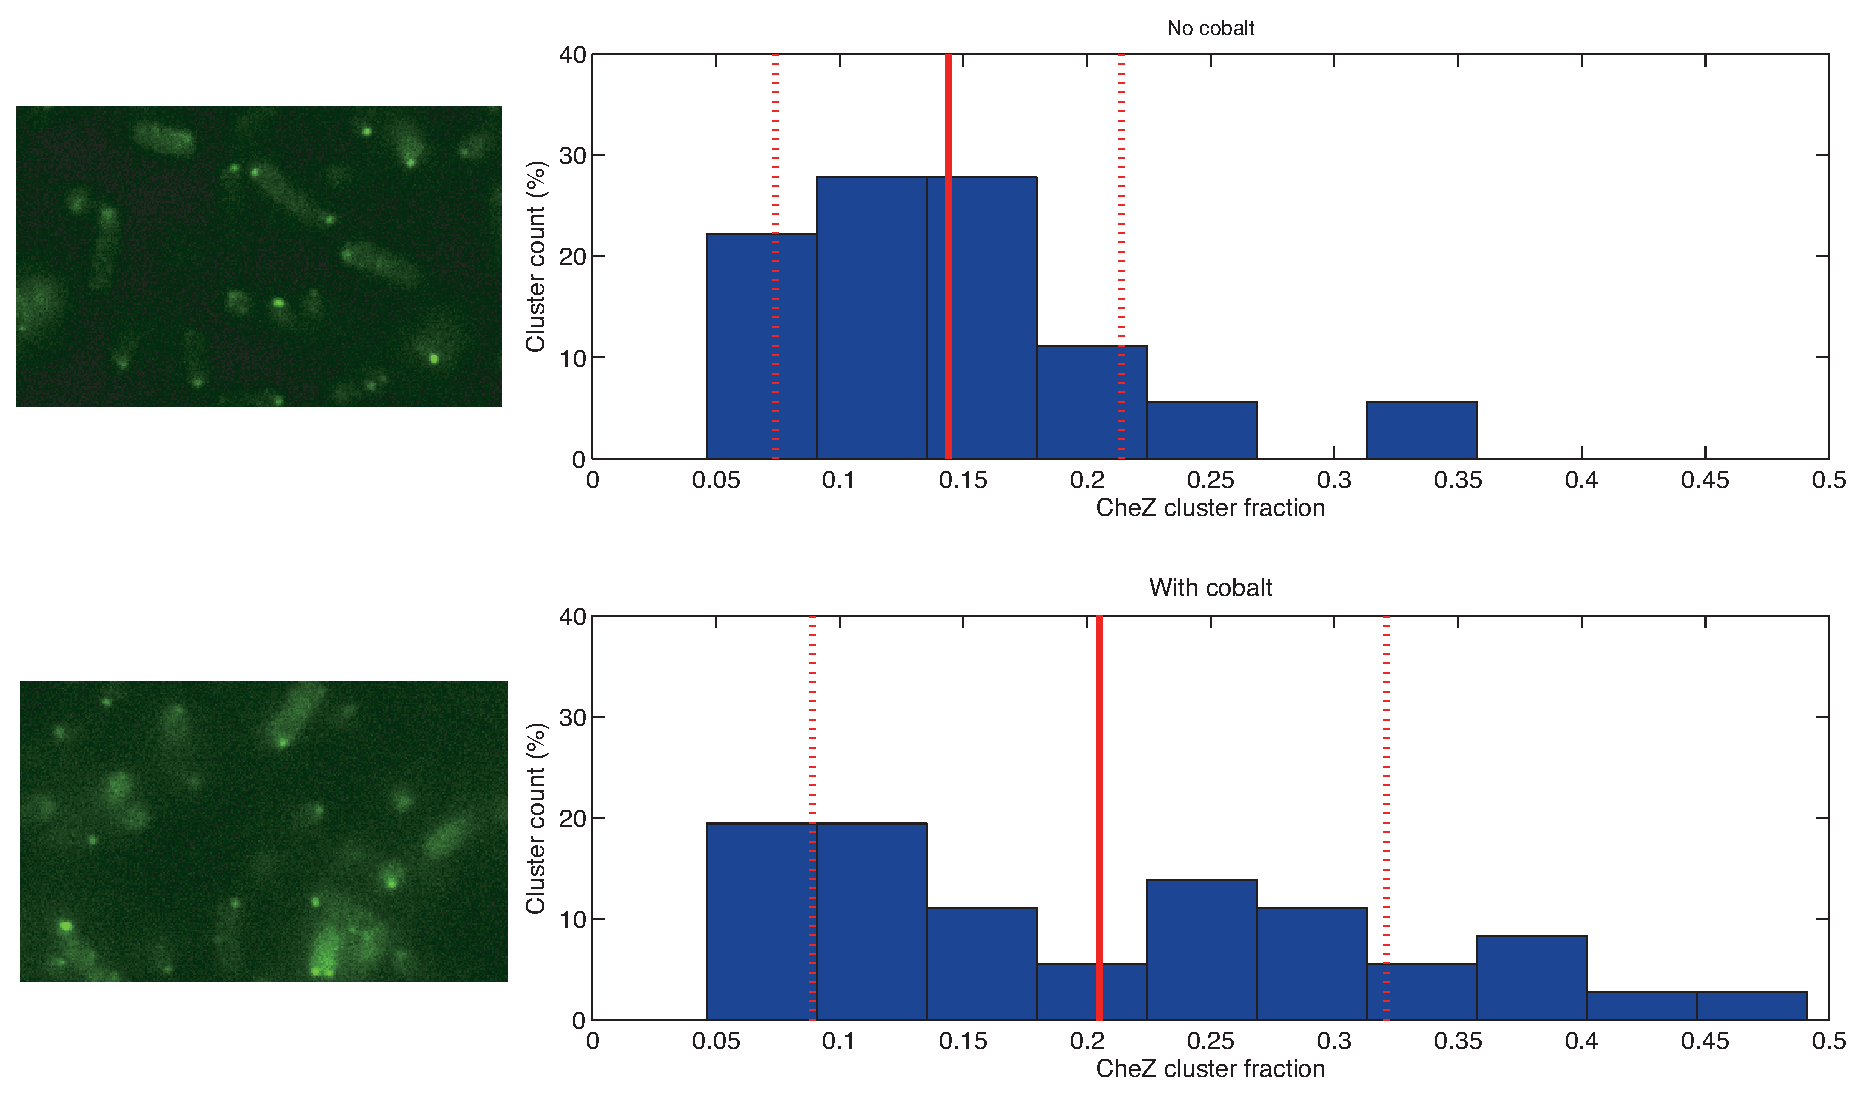
\includegraphics[scale=0.65, trim=0 300 0 40, clip=true]{\docroot results/figs/nikonb.eps}
	\label{fig:results:nikon:nocobalt}
}\\
\subfloat[With cobalt, \(n=36, \mu=0.205, \sigma=0.116\)]{
	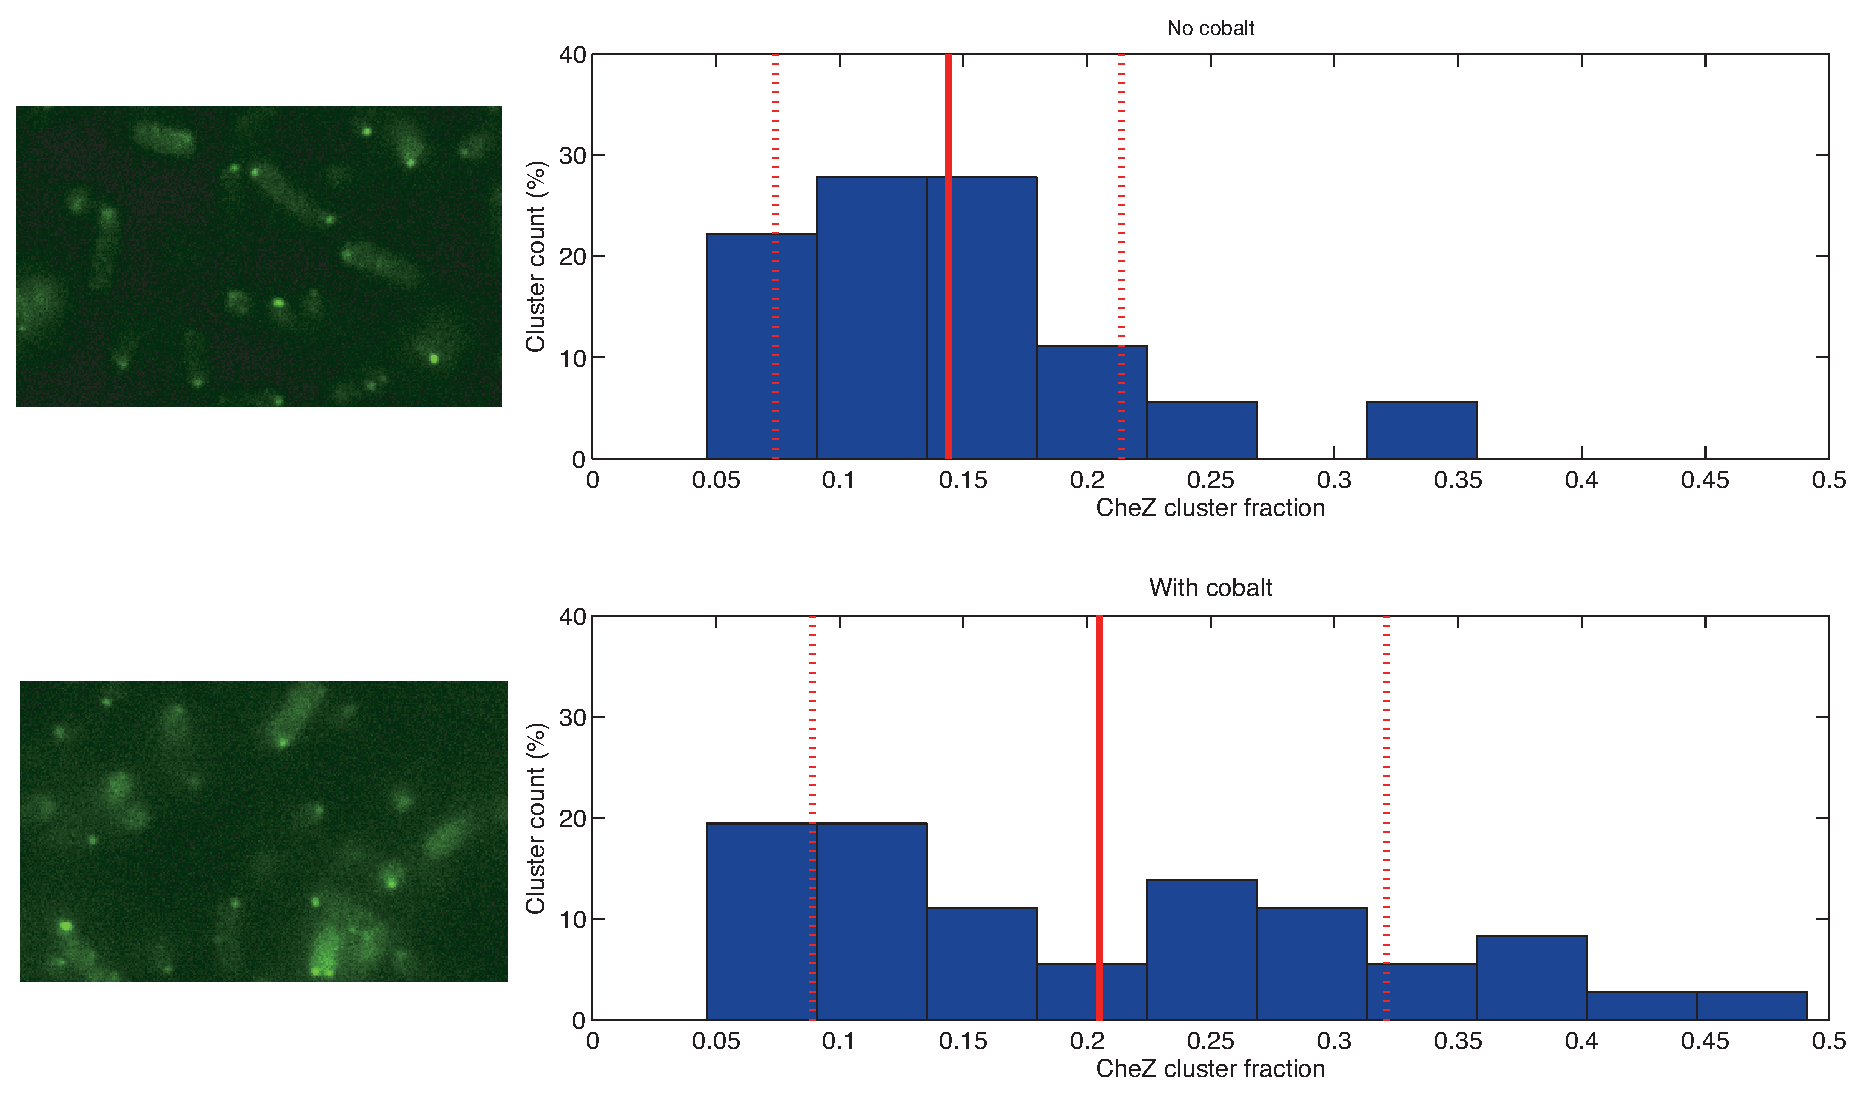
\includegraphics[scale=0.65, trim=0 30 0 310, clip=true]{\docroot results/figs/nikonb.eps}
	\label{fig:results:nikon:cobalt}
}
\caption{Histograms of CheZ cluster fraction (fraction of CheZ protein in cell localised in the polar cluster). Solid red line marks mean average, dashed lines \(\pm\sigma\).}
\label{fig:results:nikon}
\end{center}
\end{figure}

\subsubsection{Confocal Microscopy}
\label{sec:results:cs:confocal}
These experiments were performed on a Zeiss confocal microscope, the use of which was kindly given to us by Alessandro Esposito at the Hutchison MRC. Ten images were taken each from a slide of cells prepared with and without cobalt.

\begin{figure}[h!]
\begin{center}
\subfloat[No cobalt, \(n=1222, \mu=0.185, \sigma=0.068\)]{
	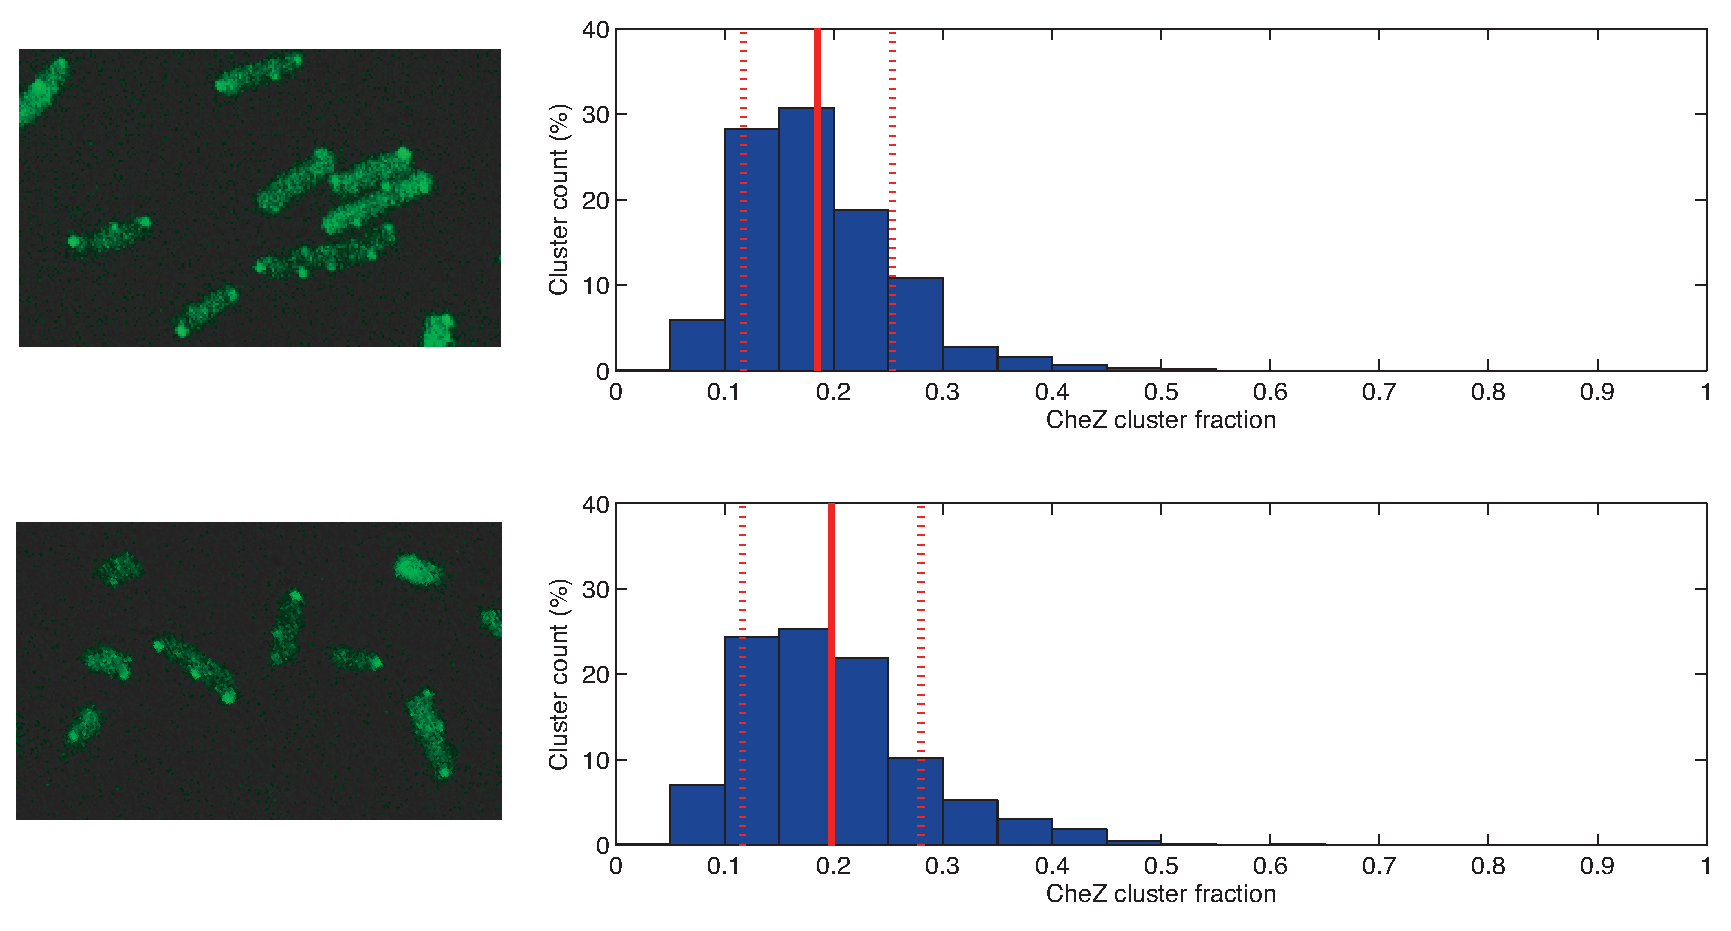
\includegraphics[scale=0.65, trim=0 250 0 30, clip=true]{\docroot results/figs/zeiss.eps}
	\label{fig:results:zeiss:nocobalt}
}\\
\subfloat[With cobalt, \(n=644, \mu=0.198, \sigma=0.082\)]{
	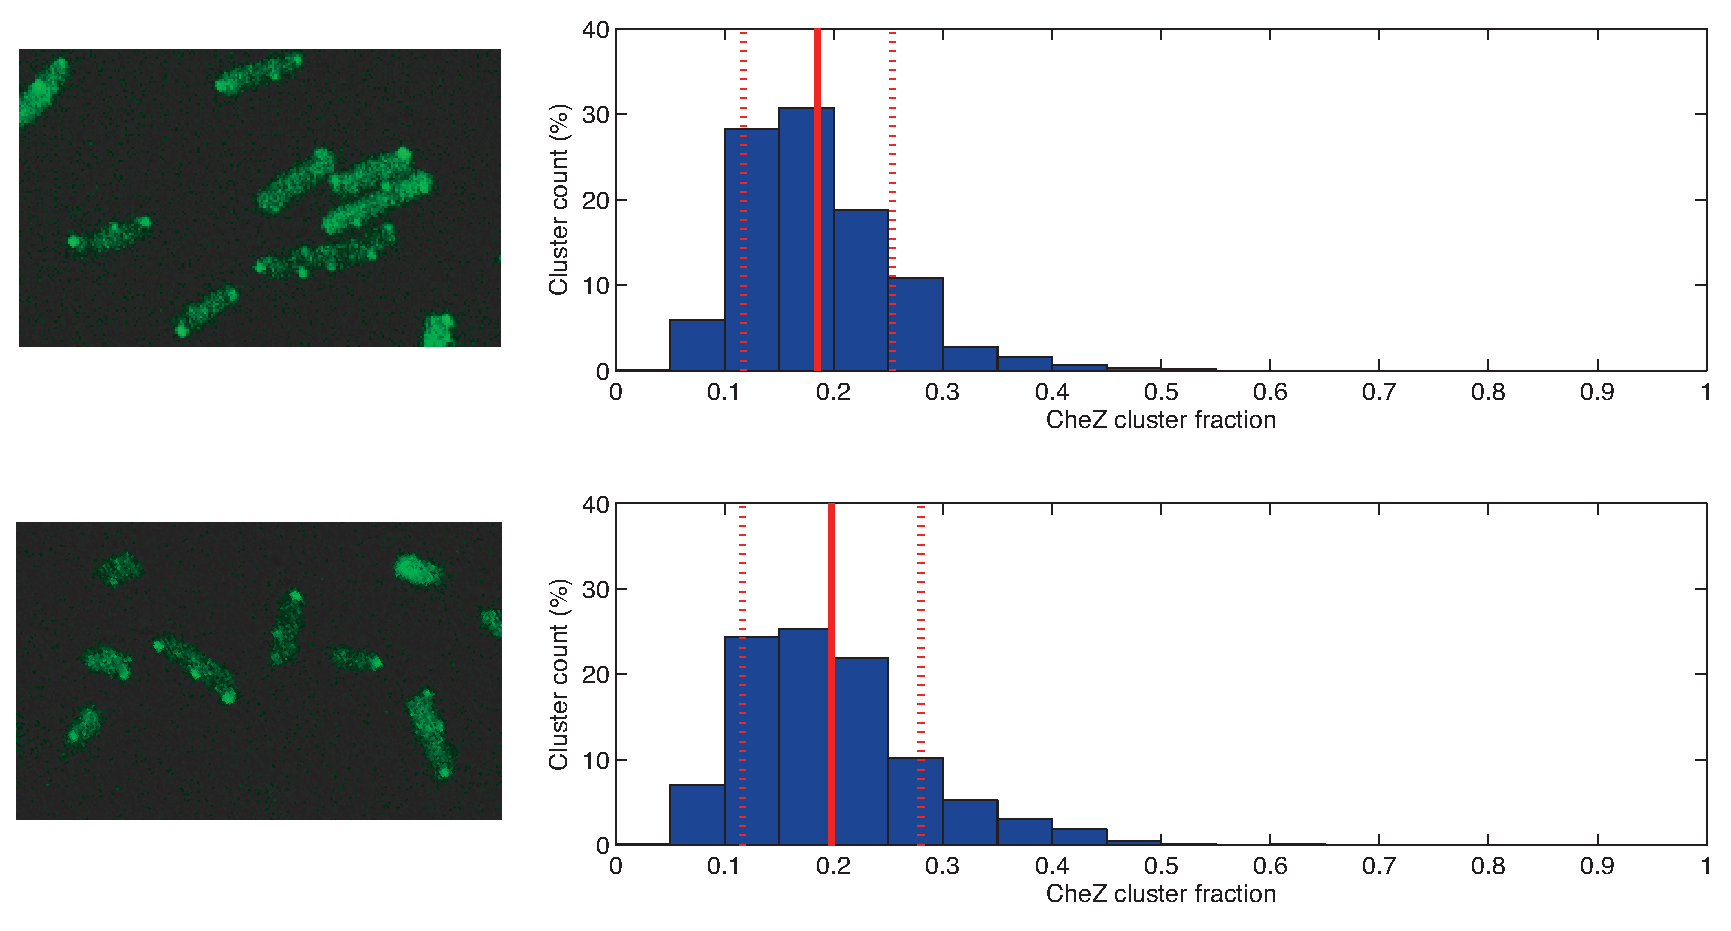
\includegraphics[scale=0.65, trim=0 20 0 260, clip=true]{\docroot results/figs/zeiss.eps}
	\label{fig:results:zeiss:cobalt}
}
\caption{Histograms of CheZ cluster fraction (fraction of CheZ protein in cell localised in the polar cluster). Solid red line marks mean average, dashed lines \(\pm\sigma\). \(p\) value \(=0.0349\%\).}
\label{fig:results:zeiss}
\end{center}
\end{figure}

\end{document}